\chapter{Geoteknik}

For at kunne dimensionere et fundament, er det vigtigt at have en grundlæggende viden om det materiale, der arbejdes med, altså jord, samt dets egenskaber og styrkeegenskaber. I det følgende vil der derfor foretages en beskrivelse af jord og dets styrkeparametre.
\newline \indent{     }  Efterfølgende….

\section{Jord}
\subsection{Beskrivelse af jord og jordtyper}
Jord er en massebetegnelse, da der findes mange forskellige typer af jordarter. Der findes to hovedgrupper af jord; rene mineraljordarter og organiske jordarter. 
\newline \indent{     }  De rene mineraljordarter kan være sorterede eller usorterede. Mineraljordarterne kan blive sorteret ved vand- og vindaflejring, og kan blive til det, der kendes som grus, sand, silt og ler. De usorterede mineraljordarter aflejres primært ved gletsjeraflejring, og betegnes som morænejordarter kaldet till.\citep{jordarter}
\newline \indent{     }  Organiske jordarter består af organisk materiale i form af plante- eller dyrerester. Disse jordarter kendes som muld, tørv, gytje mm.\citep{miljo}
\newline \indent{     }  De forskellige jordtyper har forskellige egenskaber. Egenskaberne afhænger af kornstørrelserne, som angives ved kornets diameter, og herved kan de inddeles i kornfraktioner\citep{geoteknik}. For eksempel ses inddelingen af kornstørrelserne for nogle mineraljordarter på Figur \ref{fig:kornstorrelser} .

\begin{figure}[htbp] \centering
	\begin{minipage}[b]{0.48\textwidth}\centering
		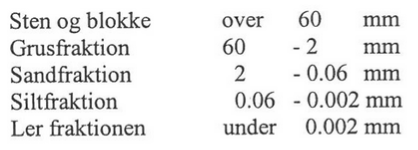
\includegraphics[width=1.0\textwidth]{billeder/kornetsdiameter.png}
		\caption{Inddeling af kornstørrelser (KILDE)}
		\label{fig:kornstorrelser}
	\end{minipage}\hfill
\end{figure}

\subsection{Jordtypernes udseende og dannelse}
Grus-  og sandjordarter skabes ved forvitring og erosion af materiale fra faste bjergarter. Materialet bliver herefter transporteret og aflejret via vind eller vand. Dette gør, at deres sammensætning bestemmes af udgangsmaterialet, men i lige så høj grad af transportmåden og transporttiden. Transporttiden kan gøre, at bløde dele af materialet opløses, samt at materialet får en afrundet kornform, og dette giver en mindre friktionsvinkel. Den relative store kornstørrelse ved grus og sandjordarter gør, at de har et groft porenet, hvilket medvirker, at vandet bevæger sig let i materialet,  dvs. at permeabiliteten er stor. Samtidig ved belastning af materialet sker der en vandudpresning, hvilket er en hurtig konsolidering.\citep{jordarter}
\newline \indent{     }  Grus- og sandjordarters styrkeegenskaber afhænger af friktionen mellem kornene, som afhænger af kornenes lejringstæthed, materialets enskornethed og kornenes enkelte form; om de er skarpkantet eller afrundet.\citep{jordarter} 
\newline \indent{     }  Lerjordarter har alle et bestemt indhold af lermineraler. Indholdet af disse har en betydende indflydelse på lerjordartens egenskaber, også selvom de ikke udgør størstedelen af jordarten. Lermineralerne bliver til ved en kemisk forvitring af faste bjergarter. De mest betydende grupper af lermineraler er; kaolinit, smectit, illit og chlorit. Den kemiske sammensætning af lermineralerne kan være meget forskellige og har en stor betydning for de fysiske egenskaber.\citep{jordarter} Alle lermineralerne kan optage vandmolekyler, hvilket gør, at lerjordarter kan indeholde meget vand. Betydningen af vandet kan fysisk ses ved tilsætning af vand til lerjordarterne, som gør at de sveller og ligeledes svinder ved tørring. Hvis lerpartiklerne er placeret med kort afstand til hinanden, vil dette give jordarten en større styrke.\citep{jordarter}  Ved at smadre jordarten formindskes jordartens styrke, men en del af denne styrke kan jordarten genvinde efter noget tid. \citep{jordarter}
\newline \indent{     }  Morænejordarter er typisk usorterede mineraljordarter, og kan derfor bestå af flere forskellige kornstørrelser. Fordelingen af dem kan skifte inden for korte afstande. Morænejordarter har normalt gode styrke- og deformationsegenskaber, da de er forbelastede.\citep{jordarter}
\newline \indent{     }  Organiske jordarters egenskaber er afhængige af de organiske bestanddeles art. De forskellige typer af organiske jordarter bliver dannet forskellige steder. Tørv og gytje bliver for eksempel dannet i moser, søer, bugter, fjorde mm, og dets styrke er ikke høj. Dette skyldes, at disse indeholder store mængder vand, da der ikke er faste partikler og at organiske materialer forsvinder med tiden. \citep{jordarter}

\subsection{Jords styrke og stivhed}
Jord betragtes, på lige fod med beton, stål osv, som et byggemateriale, da dens fysiske egenskaber er vigtige for konstruktions dimensionering.\citep{DGF} 
\newline \indent{     }  Jordarterne har meget forskellige styrker, og inden for geoteknik kan jordarterne inddeles i to forskellige typer. Den ene type er friktionsjord, for eksempel sand og grus. Den anden er kohæsionsjord med et indhold af mere end 10\% lerfraktion. 
Friktionsjord er under stabil lejring næsten usammentrykkeligt, og hvis deformationer finder sted forskydninger eller gnidninger kornene imellem.\citep{DGF}
\newline \indent{     }  I kohæsionsjord kan kornskelettet være stabilt ved åbne strukturer, men kun ved små deformationer og belastninger, afhængig af forbelastning. Ved store belastninger er disse jordarter sammentrykkelige.
\newline \indent{     }  Med hensyn til jordarters styrke, benyttes begreberne træk- og trykstyrke normalvis ikke. I stedet for anvendes forskydningsstyrken. Denne anvendes da der ved brud i jorden, sker en forskydning af jordmasser. Når der sker et sådant brud, virker der normal- og forskydningsspændinger langs brudlinjen.\citep{geoteknik} Forskydningsspændingen virker som en reaktion på jordmassens bevægelse nedad, og derfor er denne rettet skråt op ad. Normalspændingen, også kaldet brudspændingen, står vinkelret på brudlinjen, og regnes positiv ved tryk. Det vil være fordelagtigt at dele spændingen op i to bidrag; den effektive brudspænding og poreovertryk, som er trykket i porerne\citep{geoteknik}. Dette er illustreret på Figur \ref{fig:poretrykket}. 

\begin{figure}[htbp] \centering
	\begin{minipage}[b]{0.48\textwidth}\centering
		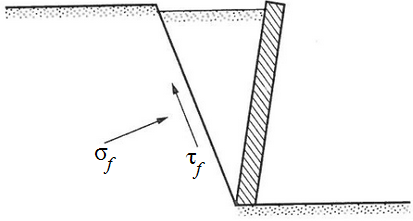
\includegraphics[width=1.0\textwidth]{billeder/poretrykket.png}
		\caption{BILLEDTEKST}
		\label{fig:poretrykket}
	\end{minipage}\hfill
\end{figure}

For at finde brud i jord bruges en skæreboks, som er illustreret på Figur \ref{fig:forskudningsspanding}. Jordprøven lukkes inde i en kasse, som lodret kan lastes med en varierende normalkraft. Kassen er delt vandret på midten, og ved at trække i øverste halvdel skabes et veldefineret vandret brud. Derved kan værdierne for brud- og forskydningsspænding måles.\citep{DGF}

\begin{figure}[htbp] \centering
	\begin{minipage}[b]{0.48\textwidth}\centering
		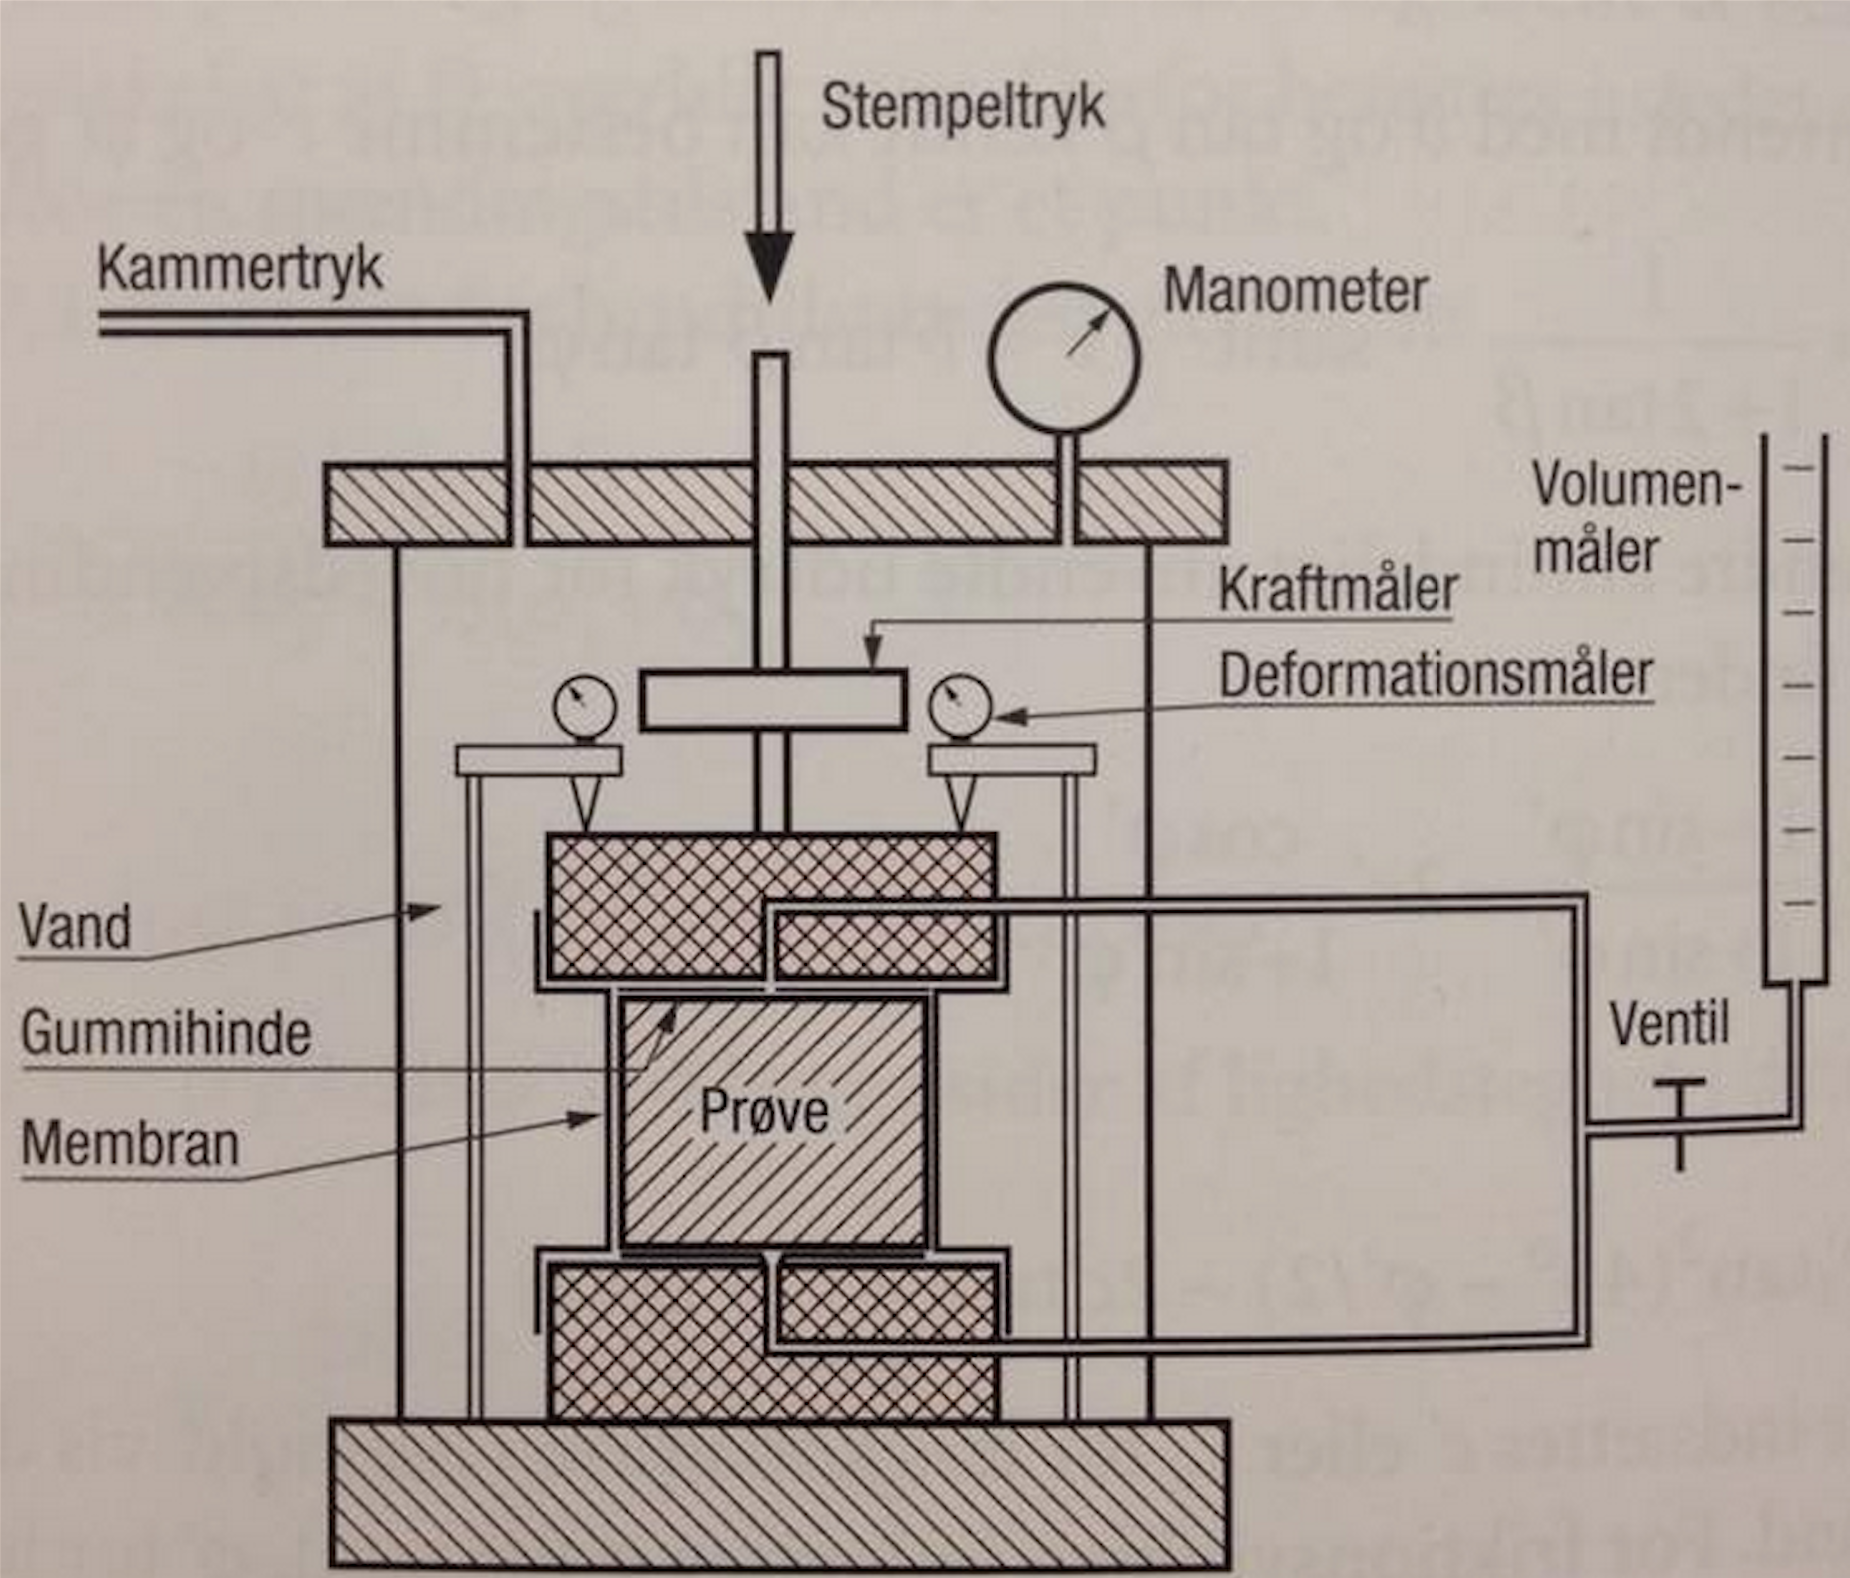
\includegraphics[width=0.8\textwidth]{billeder/forskud.png}
		\caption{BILLEDTEKST}
		\label{fig:forskudningsspanding}
	\end{minipage}\hfill
\end{figure}

\indent{     }  I kassen er jordprøven isoleret fra toppen og bunden via filtersten. Disse gør det muligt at kontrollere poretrykket, og således bestemme den effektive brudspænding. Ved forsøget findes der, at forskydningsspændingen består af to dele; kohæsionen og et friktionsbidrag. Kohæssionen er et konstant bidrag, og friktionsbidraget er proportionalt med den effektive brudspændning. Sammenhængen her kaldes for jordens brudbetingelse.\citep{geoteknik}

\section{Fundering}
Et fundament er en del af et bygværk, hvor formålet er at overføre belastningen fra bygningen til underliggende, bærende jordlag. Der findes mange forskellige funderingsmetoder, for eksempel pælefundering og direkte fundering, og kan i nogle tilfælde kombineres. De to mest almindelige funderingsmetoder er pæle- og direkte fundering, hvilke vil blive omtalt i denne rapport.
\newline \indent{     }  Ved direkte fundering støbes fundamentet direkte på terrænet, hvor de bæredygtige jordlag findes relativt tæt under bygningen. Belastningen overføres fra bygningen til jorden igennem vandrette flader. Belastningen på fundamentfladen udgøres af fundamentets egenvægt og bygingens belastning. Hvis belastningen virker på en lang fundamentflade med konstant bredde, er der tale om et stribefundament, der som regel bruges ved fundering af bærende vægge. Modsætningen hertil er punktfundamenter, som er rektangulære eller kvadratiske, og disse bruges for eksempel ved fundering af master, søjler og skorstene \citep[ s. 221]{geoteknik}. Stribefundamentet og punktfundamentet er illustreret på Figur \ref{fig:fundament}. 

\begin{figure}[htbp] \centering
	\begin{minipage}[b]{0.48\textwidth}\centering
		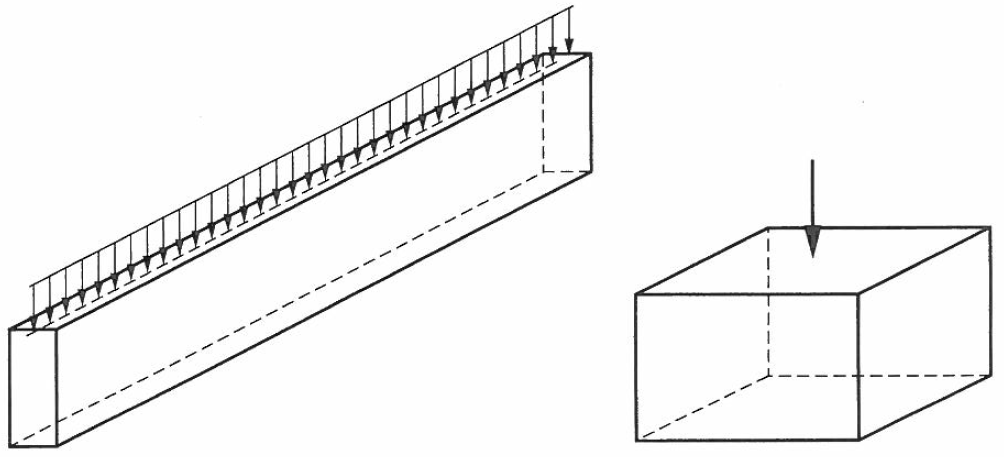
\includegraphics[width=1.0\textwidth]{billeder/fundament.png}
		\caption{Stribefundament og enkeltfundament \citep[ s. 221]{geoteknik}}
		\label{fig:fundament}
	\end{minipage}\hfill
\end{figure}

\indent{     }  Hvis de bæredygtige jordlag ligger mere end 4-5 meter under bygingen, anvendes ofte pælefundering. Ved pælefundering er søjleformede pæle af træ, beton, og/eller stål, rammet, presset, vibreret eller udstøbt i jorden. Pæleformen er normalt cylindrisk med cirkulært eller kvadratisk tværsnit. Pælefundering benyttes blandt andet når de bærende jordlag ligger så dybt, at direkte fundering vil blive uøkonomisk \citep[ s. 355]{geoteknik}.
\newline
\newline
Valg af funderingsmetode for tilbygningen til Strøybergs Palæ afhænger af jordbunds- og grundvandsforhold samt de belastninger, som konstruktionen er udsat for \citep[ s. 355]{geoteknik}. Det er derfor nødvendigt at have kendskab til områdets geologi omkring Strøybergs Palæ, og at tolke på de boreprofiler, der bliver udført på stedet, hvilket vil gøres i forsøgene i Afsnit 8.4. 

\section{Antagelser}
Idét Aalborg er funderet på meget blødt ler, benyttes boreprofiler fra Hals/Hou, og det antages, at disse boreprofiler er fra området ved Strøybergs Palæ. 
\newline \indent{     }  Forsøgene er udført på baskarpsand fra Sverige, hvilket antages at være sandet fra boreprofilerne.

\section{Forsøg}
For at bestemme styrkeparametre for jorden udføres laboratorieforsøg, der bruges ved dimensionering af fundamentet.
\newline
\newline
Formålet med forsøgene er at bestemme friktionsvinklen, givet ved: 

\begin{center}
	$\varphi = 30^\circ - \frac{3}{U} + (14 - \frac{4}{U}) I_D$
\end{center}

\begin{itemize}
	\item[-] U: Uensformighedtal
	\item[-] $I_D$: Relativ lejringstæthed
\end{itemize}

Friktionsvinklen $\varphi$ er et mål for jords styrke, og skønnes ud fra sigteanalyse samt løs og fast lejring. Ved hjælp af nedenstående fire forsøg bestemmes friktionsvinklen, idét uensformighedstallet og den relative lejringstæthed bestemmes herudfra: 
\begin{enumerate}
	\item Vandindhold
	\item Sigteanalyse
	\item Kornvægtfylde
	\item Løs og fast lejring
\end{enumerate}
Tabeller over resultater, fremgangsmåde, apparaturliste samt fejlkilder for de enkelte forsøg findes i bilag A-D.

\subsection{Forsøg 1: Vandindhold}
Formålet med forsøget “vandindhold” er at finde vandindholdet \textit{w} i jordprøven. Vandindholdet er defineret som jordens vægttab i \% af tørvægten ved tørring i et varmeskab ved en temperatur på 105$^{\circ}$C. For naturligt forekommende jordarter kan vandindholdet ligge mellem nul og flere hundrede procent.
\newline
\newline
Vandindholdet beregnes ved:

\begin{center}
	$w = \frac{W_w}{W_s}\cdot 100\% = \frac{(W+sk)-(W_s+sk)}{(W_s+sk)-sk}\cdot 100\%$
\end{center}

\begin{itemize}
	\item[-] $W_w$: Vægten af vandet i prøven [g]
	\item[-] $W_s$: Vægten af det tørrede materiale [g]
	\item[-] W: Vægten af prøven før tørring [g]
	\item[-] sk: Vægten af skålen [g]
\end{itemize}

Forsøget er udført to gange. De fundne værdier for de to udførte forsøg ses i tabellen i Bilag A. Vandindholdet for de to forsøg er beregnet til:

\begin{center}
	Forsøg 1: $w = \frac{81,\!02 g - 80,\!99 g}{80,\!99 g - 3,\!07 g}\cdot 100\% = 0,\!04\%$
\end{center}

\begin{center}
	Forsøg 2: $w = \frac{89,\!83 g - 89,\!79}{89,\!79 g - 3,\!11 g}\cdot 100\% = 0,\!05\%$
\end{center}

Ud fra de opnåede resultater, kan det konkluderes, at det benyttede materiale vurderes at være tørt og det meget lille vandindhold har ikke indflydelse på de øvrige resultater.
\newline \indent{     }  Til videre beregninger benyttes gennemsnittet for vandindholdet for forsøg 1 og forsøg 2, som er $0,\!04$\%. Dette skal bruges som et rent tal, som er $0,\!0004$. 

\subsection{Forsøg 2: Sigteanalyse}
Formålet med “sigteanalyse” er at bestemme jordkornenes vægtmæssige fordeling efter størrelse i sand- og grusfraktion, for at beregne uensformighedstallet \textit{U} for jorden:

\begin{center}
	$U = \frac{d_{60}}{d_{10}}$
\end{center}

\begin{itemize}
	\item[-] $d_{60}$: 60\%-fraktilen
	\item[-] $d_{10}$: 10\%-fraktilen
\end{itemize}

Uensformighedstallet fortæller, hvor velsorteret jorden er:

\begin{itemize}
	\item[-] Velsorteret: $U < 2$
	\item[-] Sorteret: $2 < U < 3,\!5$
	\item[-] Ringe sorteret: $3,\!5 < U < 7$
	\item[-] Usorteret: $U > 7$
\end{itemize}

Forsøget er udført to gange, og der er derfor lavet en sigtekurve for hvert forsøg, og uensformighedstallet er udregnet for begge forsøg. 
\newline \indent{     }  Det procentvise gennemfald i hver sigte er beregnet, og herudfra fås sigtekurverne vist på Figur \ref{fig:sigtekurve1} og Figur \ref{fig:sigtekurve2}. Værdierne der er brugt til at finde det procentvise gennemfald findes i Bilag B. 

\begin{figure}[htbp]
		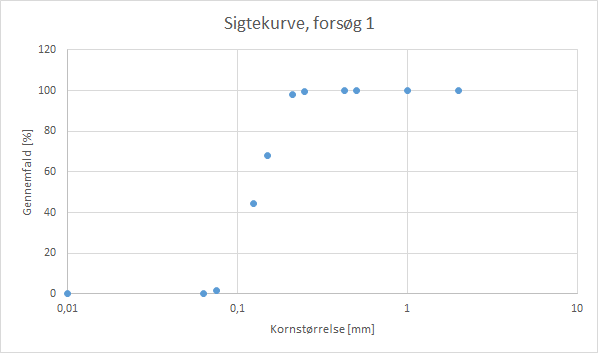
\includegraphics[width=1.0\textwidth]{billeder/sigtekurve1.png}
		\caption{Sigtekurve til forsøg 1}
		\label{fig:sigtekurve1}
\end{figure}

\begin{figure}[htbp]
		\centering
		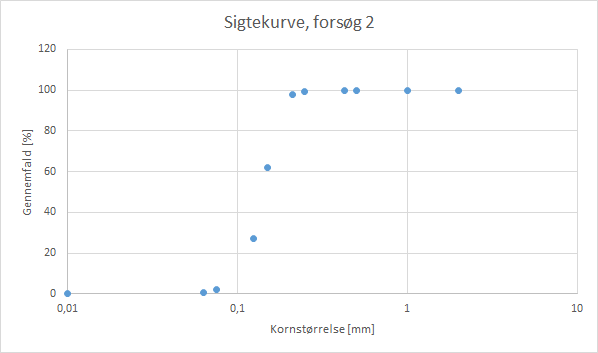
\includegraphics[width=1.0\textwidth]{billeder/sigtekurve2.png}
		\caption{Sigtekurve til forsøg 2}
		\label{fig:sigtekurve2}
\end{figure}

Uensformighedstallet for begge forsøg er beregnet, ved at lave lineær regression imellem henholdsvis 10\% og 60\% og derved finde 10\%-fraktilen og 60\%-fraktilen.
\newline
\newline
Ved det første udførte forsøg er 10\%-fraktilen fundet ved at lave lineær regression imellem sigte med maskestørrelse $0,\!075$ mm og $0,\!125$ mm, hvor følgende ligning fremgår: 

\begin{center}
	$y = 862,\!42x - 63,\!223$
\end{center}

For at finde 60\%-fraktilen er der lavet lineær regression imellem sigte med maskestørrelse $0,\!125$ mm og $0,\!15$ mm, hvor følgende ligning fremgår:

\begin{center}
	$d_{60}=937,\!12x - 72,\!56mm$
\end{center}

Ved forsøg 1 er 10\%-fraktilen og 60\%-fraktilen hermed beregnet til: 
\begin{center}
	$d_{10} = 0,\!08$ og $d_{60} = 0,\!14mm$
\end{center} 

Uensformighedstallet i forsøg 1 er derved:
\begin{center}
	$U = \frac{0,\!14}{0,\!08} = 1,\!67$
\end{center}

Ved forsøg 2 er 10\%-fraktilen, 60\%-fraktilen og uensformighedstallet beregnet til:
\begin{center}
	$d_{10} = 0,\!91$ og $d_{60} = 0,\!15$ og $U = \frac{0,\!15}{0,\!91} = 1,\!64$
\end{center} 
Uddybbende beregninger er vist i Bilag B.

Til videre beregninger benyttes gennemsnittet af uensformighedstallet for forsøg 1 og forsøg 2, som er $1,\!65$. Dette tal fortæller, at jorden er velsorteret, idet $U<2$. 

\subsection{Forsøg 3: Kornvægtfylde}
Formålet med “kornvægtfylde” er at finde den relative densitet $d_s$, også kaldet kornvægtfylden, for jordprøven. For jordarter uden organisk indhold kan kornvægtfylden variere fra $2,\!65$ for rent kvartsand til $2,\!85$ for visse lermineraler. I dette forsøg søges altså et resultat der ligger så tæt på $2,\!65$ som muligt.
\newline
\newline
Kornvægtfylden beregnes ved:

\begin{center}
	$d_s = \frac{W_s \rho_w^t}{(W_s + W_2 - W_1)\rho_w^{4^{\circ}}}$
\end{center}

\begin{itemize}
	\item[-] $W_s$: Vægten af tørt kornmateriale [g]
	\item[-] $p_w^t$: Densitet af luftfrit demineraliseret vand ved målte temperatur $[\frac{g}{cm^3}]$
	\item[-] $W_2$: Vægten af pyknometeret fyldt med luftfrit demineraliseret vand [g]
	\item[-] $W_1$: Vægten af pyknometer fyldt med prøve og luftfrit demineraliseret vand [g]
	\item[-] $\rho_w^{4^{\circ}}$: Densitet af luftfrit demineraliseret vand ved $4^{\circ}$, som er $1 \frac{g}{cm^3}$
\end{itemize}

Forsøget er udført to gange, og resultater for de to forsøg kan findes i Bilag C. Kornvægtfylden for de to forsøg er beregnet til:

\begin{center}
	Forsøg 1: $d_{s} = \frac{161,\!27 g \cdot 0,\!998 \frac{g}{cm^3}}{(161,\!27 g + 641,\!16 g - 728,\!89 g)\cdot 1 \frac{g}{cm^3}} = 2,\!19$
\end{center}
\begin{center}
	Forsøg 2: $d_{s} = \frac{150,\!06 g \cdot 0,\!998 \frac{g}{cm^3}}{(150,\!06 g + 615,\!97 g - 709,\!40 g)\cdot 1 \frac{g}{cm^3}} = 2,\!64$
\end{center} 

Resultatet fra forsøg 2 anvendes til videre beregninger, fordi resultatet fra forsøg 1 vurderes til at være for langt fra den ønskede værdi på $2,\!65$. Grunden til den store afvigelse kan skyldes, at der blev anvendt ca. 161 g i forhold til, at der kun skulle være anvendt 150 g.

\subsection{Forsøg 4: Løs og fast lejring}
Formålet med “løs og fast lejring” er at finde jordens relative lejringstæthed $I_D$. Lejringstætheden er et tal, som vokser fra 0 til 1, når lejringstætheden varierer fra den løseste til den fasteste lejring.
\newline
\newline
$I_D$ bestemmes ved:

\begin{center}
	$I_D = \frac{e_{max} - e_{in situ}}{e_{max} - e_{min}}$
\end{center}

\begin{itemize}
	\item[-] $e_{min}$: jordens gennemsnitlige poretal for den fasteste lejring 
	\item[-] $e_{max}$: jordens gennemsnitlige poretal for den løseste lejring
	\item[-] $e_{in situ}$: jordens naturlige poretal 
\end{itemize}

Poretallet \textit{e}, for henholdsvis den løseste og fasteste lejring beregnes ved:

\begin{center}
	$e = \frac{d_s \rho_w  V}{W_s} - 1$
\end{center}

\begin{itemize}
	\item[-] $d_s$: kornvægtfylde [rent tal], som er fundet i forsøg 3: kornvægtfylde, til $2,\!64$ 
	\item[-] $\rho_w$: Vands densitet på $1 \frac{g}{cm^3}$
	\item[-] V: Volumen af materialet $[cm^3]$
	\item[-] $W_s$: Vægten at tørt kornmateriale [g]
\end{itemize}
 
Der er udført fire forsøg for henholdsvis den løseste og den fasteste lejring. Poretallet for hvert enkelt forsøg kan aflæses i Bilag D.
Det gennemsnitlige poretal er:

\begin{center}
	$e_{min} = \frac{0,\!595 + 0,\!571 + 0,\!573 + 0,\!569}{4} = 0,\!577$
\end{center}

\begin{center}
	$e_{max} = \frac{0,\!873 + 0,\!875 + 0,\!874 + 0,\!873}{4} = 0,\!874$
\end{center}

Herefter bestemmes jordens naturlige poretal $e_{in situ}$ ved:

\begin{center}
	$e_{in situ} = (1 + w) \frac{d_s  \rho_w  V}{W_s} - 1$
\end{center}

\begin{itemize}
	\item[-] w: det naturlige vandindhold [rent tal], fra forsøg 1: vandindhold, til $0,\!0004$ 
\end{itemize}

Dette er beregnet til:

\begin{center}
	$e_{in situ} = (1+0,\!0004) \cdot \frac{2,\!64 \cdot 1,\!00 \frac{g}{cm^3} \cdot 269,\!39 cm^3}{421,\!4 g} - 1 = 0,\!691$
\end{center}

Slutteligt kan den relative lejringstæthed $I_D$ bestemmes til:

\begin{center}
	$I_D = \frac{0,\!874 - 0,\!691}{0,\!874 - 0,\!577} = 0,\!617$
\end{center}

\subsection{Friktionsvinklen}
Efter udførelsen af de fire forsøg kan friktionsvinklen beregnes til:

\begin{center}
	$\varphi = 30^\circ - \frac{3}{1,\!65} + (14 - \frac{4}{1,\!65}) \cdot 0,\!619 = 35,\!3^\circ$
\end{center}

I Figur \ref{fig:friktionsvinkel} ses det, at der kan trækkes henholdsvis 3 eller 5 grader fra friktionsvinklen eller lægges 1 eller 2 grader til friktionsvinkel, alt efter jordens type. Baskarpsandkornene er vurderet til at være afrundede, og derfor trækkes der 3 grader fra den friktionsvinkel, som er fundet ovenfor, og der fås en friktionsvinkel på $32,\!3^\circ$. 
\newline
\newline
Friktionsvinklen sammenlignes med værdierne fra Figur \ref{fig:friktionsvinkel}. Der aflæses ud fra de $32^{\circ}$, hvor graderingen aflæses som værende enskornet, og lejringstætheden aflæses som værende middel. Hvilket vurderes til at passe med, at det anvendte sand blev vurderet til at være enskornet.

\begin{figure}[htbp] \centering
	\begin{minipage}[b]{0.48\textwidth}\centering
		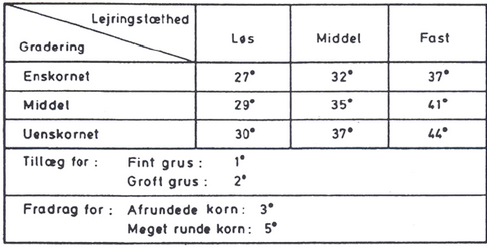
\includegraphics[width=1.2\textwidth]{billeder/friktionsvinkel.png}
		\caption{Friktionsvinkel \citep[ s. 170]{geoteknik}}
		\label{fig:friktionsvinkel}
	\end{minipage}\hfill
\end{figure}
